%!TEX root = ../Thesis.tex
%% Basierend auf TeXnicCenter-Vorlage von Mark Müller
%%                      Willi Nüßer
%%                      Waldemar Penner     
%%                      Ulrich Reus
%%                      Frank Plass
%%                      Oliver Tribeß 
%%                      Daniel Hintze     
%%%%%%%%%%%%%%%%%%%%%%%%%%%%%%%%%%%%%%%%%%%%%%%%%%%%%%%%%%%%%%%%%%%%%%%

% Wählen Sie die Optionen aus, indem Sie % vor der Option entfernen  
% Dokumentation des KOMA-Script-Packets: scrguide

%%%%%%%%%%%%%%%%%%%%%%%%%%%%%%%%%%%%%%%%%%%%%%%%%%%%%%%%%%%%%%%%%%%%%%%
%% Optionen zum Layout des Artikels                                  %%
%%%%%%%%%%%%%%%%%%%%%%%%%%%%%%%%%%%%%%%%%%%%%%%%%%%%%%%%%%%%%%%%%%%%%%%
\documentclass[%
paper=A4,         % alle weiteren Papierformat einstellbar
fontsize=12pt,    % Schriftgröße (12pt, 11pt (Standard))
BCOR=12mm,         % Bindekorrektur, bspw. 1 cm
DIV=14,            % breiter Satzspiegel
parskip=half*,    % Absatzformatierung s. scrguide 3.1
headsepline,      % Trennline zum Seitenkopf  
%footsepline,     % Trennline zum Seitenfuß
%normalheadings,  % Überschriften etwas kleiner (smallheadings)
listof=totoc,     % Tabellen & Abbildungsverzeichnis ins Inhaltsverzeichnis      
%bibtotoc,        % Literaturverzeichnis im Inhalt 
%draft            % Überlangen Zeilen in Ausgabe gekennzeichnet
footinclude=false,% Fußzeile in die Satzspiegelberechnung einbeziehen 
headinclude=true, % Kopfzeile in die Satzspiegelberechnung einbeziehen 
final             % draft beschleunigt die Kompilierung
]
{scrartcl}

%\setuptoc{toc}{totoc} % Inhaltsverzeichnis ins Inhaltsverzeichnis

% Neue Deutsche Rechtschreibung und Deutsche Standardtexte
\usepackage[ngerman]{babel} 

% Umlaute können verwendet werden
\usepackage[utf8]{inputenc}   

% Echte Umlaute
\usepackage[T1]{fontenc} 

% Latin Modern Font, Type1-Schriftart für nicht-englische Texte
\usepackage{lmodern} 

% 1/2-zeiliger Zeilenabstand
\usepackage[onehalfspacing]{setspace}

% Für die Defenition eigener Kopf- und Fußzeilen
\usepackage{fancyhdr} 

% Listing Placement
\usepackage{float}

% Für die Verwendung von Grafiken
\usepackage[pdftex]{graphicx}

% Bessere Tabellen
\usepackage{tabularx}

% Für die Befehle \toprule, \midrule und \bottomrule, z.B. in Tabellen 
\usepackage{booktabs}

% Erlaubt die Benutzung von Farben
\usepackage{color}

% Verbessertes URL-Handling mit \url{http://...}
\usepackage{url}

% Listen ohne Abstände \begin{compactlist}...\end{compactlist}
\usepackage{paralist} 

% Ausgabe der aktuellen Uhrzeit für die Draft-Versionen
\usepackage{datetime}

% Deutsche Anführungszeichen
\usepackage[babel,german=quotes]{csquotes}

% Konfiguration der Abbildungs- und Tabellenbezeichnungen
\usepackage[format=hang, font={footnotesize, sf}, labelfont=bf, justification=raggedright,singlelinecheck=false]{caption}

% Verbessert die Lesbarkeit durch Mikrotypografie
\usepackage[activate={true,nocompatibility},final,tracking=true,kerning=true,spacing=true,factor=1100,stretch=10,shrink=10]{microtype}  

% Zitate und Quellenverzeichnis
\usepackage[
    bibstyle=authoryear,
    citestyle=authoryear-fhdw,  
    giveninits=false,         % false = Vornamen werden ausgeschrieben
    natbib=true,
    urldate=long,             % "besucht am" - Datum
    %url=false,
    date=long,                
    dashed=false, 
    maxcitenames=3,           % max. Anzahl Autorennamen in Zitaten
    maxbibnames=99,           % max. Anzahl Autorennamen im Quellenverzeichnis
    %backend=bibtex           % Ggf. für ältere Distributionen bibtex verwenden
    backend=biber
]{biblatex}
  
% Bibliograpthy
\bibliography{library/library}

% Keine Einrückung bei einem neuen Absatz 
\parindent 0pt 

% Ebenentiefe der Nummerierung
\setcounter{secnumdepth}{3}

% Gliederungstiefe im Inhaltsverzeichnis 
\setcounter{tocdepth}{3} 

% Tabellen- und Abbildungsverzeichnis mit Bezeichnung:
\usepackage[titles]{tocloft}

% Sourcecode-Listings
\usepackage{listings}

% Bestimmte Warnungen unterdrücken
% siehe http://tex.stackexchange.com/questions/51867/koma-warning-about-toc
% \usepackage{scrhack} % Removed to avoid missing package error

%% http://tex.stackexchange.com/questions/126839/how-to-add-a-colon-after-listing-label
\makeatletter
\begingroup\let\newcounter\@gobble\let\setcounter\@gobbletwo
  \globaldefs\@ne \let\c@loldepth\@ne
  \newlistof{listings}{lol}{\lstlistlistingname}
\endgroup
\let\l@lstlisting\l@listings
\makeatother

\renewcommand*\cftfigpresnum{Abbildung~}
\renewcommand*\cfttabpresnum{Tabelle~}
\renewcommand*\cftlistingspresnum{Listing~}
\renewcommand{\cftfigaftersnum}{:}
\renewcommand{\cfttabaftersnum}{:}
\renewcommand{\cftlistingsaftersnum}{:}
\settowidth{\cftfignumwidth}{\cftfigpresnum 99~\cftfigaftersnum}
\settowidth{\cfttabnumwidth}{\cfttabpresnum 99~\cftfigaftersnum}
\settowidth{\cftlistingsnumwidth}{\cftlistingspresnum 99~\cftfigaftersnum}
\setlength{\cfttabindent}{1.5em}
\setlength{\cftfigindent}{1.5em}
\setlength{\cftlistingsindent}{1.5em}

\renewcommand\lstlistlistingname{Listingverzeichnis}
 
% Style für Kopf- und Fußzeilenfelder
\pagestyle{fancy}
\fancyhf{}
\fancyhead[R]{\leftmark}
\fancyfoot[R]{\thepage} 
\renewcommand{\sectionmark}[1]{\markboth{#1}{#1}} 
\fancypagestyle{plain}{}

% Macro für Quellenangaben unter Abbildungen und Tabellen
\newcommand{\source}[1]{{\vspace{-1mm}\\\footnotesize\textsf{\textbf{Quelle:}} \textsf{#1}\par}}

% Anpassungen der Formatierung an Eclipse-Aussehen 
% http://jevopi.blogspot.de/2010/03/nicely-formatted-listings-in-latex-with.html
%\definecolor{sh_comment}{rgb}{0.12, 0.38, 0.18 } %adjusted, in Eclipse: {0.25, 0.42, 0.30 } = #3F6A4D
%\definecolor{sh_keyword}{rgb}{0.37, 0.08, 0.25}  % #5F1441
%\definecolor{sh_string}{rgb}{0.06, 0.10, 0.98} % #101AF9
% Für Druckausgabe sollte alles schwarz sein
\definecolor{sh_comment}{rgb}{0.0, 0.0, 0.0 }
\definecolor{sh_keyword}{rgb}{0.0, 0.0, 0.0 }
\definecolor{sh_string}{rgb}{0.0, 0.0, 0.0 }

\lstset{ %
  language=Java,
  basicstyle=\small\ttfamily,
  fontadjust, 
  xrightmargin=1mm,
  xleftmargin=5mm,
  tabsize=2,
  columns=flexible,
  showstringspaces=false,
  rulesepcolor=\color{black},
  showspaces=false,showtabs=false,tabsize=2,
  stringstyle=\color{sh_string},
  keywordstyle=\color{sh_keyword}\bfseries,
  commentstyle=\color{sh_comment}\itshape,
  captionpos=t,
  lineskip=-0.3em
}

%\makeatletter
%\def\l@lstlisting#1#2{\@dottedtocline{1}{0em}{1.5em}{\lstlistingname\space{#1}}{#2}}
%\makeatother

% Anhangsverzeichnis
\usepackage[nohints]{minitoc} %Anhangsverzeichnis

\makeatletter
\newcounter{fktnr}\setcounter{fktnr}{0}
\newcounter{subfktnr}[fktnr]\setcounter{subfktnr}{0}

\renewcommand\thesubfktnr{\arabic{fktnr}.\arabic{subfktnr}}
\newcounter{anhangcounter}
\newcommand{\blatt}{\stepcounter{anhangcounter}}

\newcommand{\anhang}[1]{\setcounter{anhangcounter}{0}\refstepcounter{fktnr}
\addcontentsline{fk}{subsection}{Anhang~\thefktnr: \hspace*{1em}#1}
\subsection*{{Anhang~\thefktnr \hspace*{1em} #1 \hspace*{-1em}}}
}

\newcommand{\subanhang}[1]{\setcounter{anhangcounter}{0}\refstepcounter{subfktnr}
\addcontentsline{fk}{subsubsection}{Anhang~\thesubfktnr: \hspace*{1em}#1}
\subsubsection*{{Anhang~\thesubfktnr \hspace*{1em} #1 \hspace*{-1em}}}
}

\newcommand{\anhangsverzeichnis}{\mtcaddsection{\subsection*{Anhangsverzeichnis \@mkboth{FKT}{FKT}}}\@starttoc{fk}\newpage}

% Links im PDF
\usepackage[pdfpagemode={UseOutlines}, plainpages=false,breaklinks=true,pdfpagelabels]{hyperref}

 % Abkürzungsverzeichnis
\usepackage[automake,
			acronym,         % create list of acronyms
            nonumberlist,
            toc, 
            section,
            nopostdot,  % avoid dot after acronym
            hyperfirst=false,% don't hyperlink first use
            %sanitize=none    % switch off sanitization as description % Deprecated
            ]{glossaries}
            \newglossarystyle{mylist}{%
\setglossarystyle{long}% base this style on the list style
\renewcommand*{\glossaryentryfield}[5]{%
    \glsentryitem{##1}\textbf{##2} & ##3 \\}%
}

% Verbessert das Referenzieren von Kapiteln, Abbildungen etc.
\usepackage[german,capitalise]{cleveref}

\makeglossaries\makeglossaries 
\input{config/Abkuerzungen.tex}


%%%%%%%%%%%%%%%%%%%%%%%%%%%%%%%%%%%%%%%%%%%%%%%%%%%%%%%%%%%%%%%%%%%%%%%
%% Parameter - Hier auf die eigene Arbeit anpassen
%%%%%%%%%%%%%%%%%%%%%%%%%%%%%%%%%%%%%%%%%%%%%%%%%%%%%%%%%%%%%%%%%%%%%%%

\newcommand{\studiengang}{Wirtschaftsinformatik} 
\newcommand{\spezialisierungsbereich}{Cyber Security}
\newcommand{\martikelnummer}{101485}
\newcommand{\dokumententyp}{Bachelorthesis}
\newcommand{\abgabedatum}{10.06.2025} 
\newcommand{\ort}{Langenfeld} 
\newcommand{\koorperationsunternehmen}{Unternehmen GmbH}
\newcommand{\fhdwstandort}{Bergisch Gladbach} % oder Bielefeld, Mettmann, ...
\newcommand{\dokumententitel}{Konzeption und Implementierung eines React-Framewvorks zur flexiblen Erweiterung digitaler Datenbestände}
\newcommand{\dokumentenautor}{Thomas Benjamin Hopf}
\newcommand{\dokumentenautoradress}{Heinrichstrasse 23\\40764 Langenfeld}
\newcommand{\dokumentenpruefer}{Prof.\ Dr.\ Christian Soltenborn\\Prof.\ Dr.\ Besser}

%%%%%%%%%%%%%%%%%%%%%%%%%%%%%%%%%%%%%%%%%%%%%%%%%%%%%%%%%%%%%%%%%%%%%%%

\hypersetup{
  colorlinks=false,
  pdfborder={0 0 0},
  pdftitle=\dokumententitel,
  pdfauthor=\dokumentenautor
} 

\begin{document}

% Römische Seitennummerierung
\pagenumbering{Roman}
 
%%%%%%%%%%%%%%%%%%%%%%%%%%%%%%%%%%%%%%%%%%%%%%%%%%%%%%%%%%%%%%%%%%%%%%%
%% Titelseite
%%%%%%%%%%%%%%%%%%%%%%%%%%%%%%%%%%%%%%%%%%%%%%%%%%%%%%%%%%%%%%%%%%%%%%%

%!TEX root = ../Thesis.tex

\begin{titlepage}

\begin{center}
\includegraphics[scale=0.8]{img/fhdw}

\vspace{7mm}

\Huge{\bfseries\dokumententyp}\\

\vspace{5mm}

\LARGE{\dokumententitel}\\

\vspace{15mm}

\large{Prüfer(in):\\

\dokumentenpruefer 

\vspace{15mm}

Verfasser(in):\\

\dokumentenautor\\

\martikelnummer\\

\vspace{3mm}

\dokumentenautoradress\\

\vspace{7mm}

\studiengang\\

\spezialisierungsbereich\\

}

\enlargethispage{2em}

\vspace{15mm}

\large{Eingereicht am:\\

\abgabedatum \\

}

\end{center}


\end{titlepage}



%%%%%%%%%%%%%%%%%%%%%%%%%%%%%%%%%%%%%%%%%%%%%%%%%%%%%%%%%%%%%%%%%%%%%%%
%% Draft-Einstellungen
%%
%% Für die finale Version auskommentieren!
%%%%%%%%%%%%%%%%%%%%%%%%%%%%%%%%%%%%%%%%%%%%%%%%%%%%%%%%%%%%%%%%%%%%%%%
\fancyhead[L]{\color{red} Stand: \today~-~\currenttime}

%%%%%%%%%%%%%%%%%%%%%%%%%%%%%%%%%%%%%%%%%%%%%%%%%%%%%%%%%%%%%%%%%%%%%%%
%% Verzeichnisse
%%%%%%%%%%%%%%%%%%%%%%%%%%%%%%%%%%%%%%%%%%%%%%%%%%%%%%%%%%%%%%%%%%%%%%%


% Sperrvermerk
\include{chapter/Sperrvermerk}

% Inhaltsverzeichnis
\tableofcontents\newpage

% Glossar
\renewcommand{\glossarypreamble}{\label{glossary}}
\printglossary[style=long, title=Glossar, toctitle=Glossar] \newpage

% Abkürzungsverzeichnis
\renewcommand{\glossarypreamble}{\label{acronyms}}
\printglossary[type=acronym, style=long, title=Abkürzungsverzeichnis, toctitle=Abkürzungsverzeichnis] \newpage

\setcounter{table}{0} % printglossary erzeugt eine Tabelle, die die Nummerierung der "echten" Tabellen durcheinander bringt.

%%%%%%%%%%%%%%%%%%%%%%%%%%%%%%%%%%%%%%%%%%%%%%%%%%%%%%%%%%%%%%%%%%%%%%%
% Verzeichnisse
%%%%%%%%%%%%%%%%%%%%%%%%%%%%%%%%%%%%%%%%%%%%%%%%%%%%%%%%%%%%%%%%%%%%%%%

% Abbildungsverzeichnis
\fancyhead[R]{\listfigurename}
\listoffigures\newpage

% Tabellenverzeichnis
\fancyhead[R]{\listtablename}
\listoftables\newpage

% Quelltextverzeichnis
\fancyhead[R]{\lstlistlistingname}
\lstlistoflistings\newpage

% Kapitelüberschriften für den Arbeitstext
\fancyhead[R]{\leftmark}

%%%%%%%%%%%%%%%%%%%%%%%%%%%%%%%%%%%%%%%%%%%%%%%%%%%%%%%%%%%%%%%%%%%%%%%
%% Inhalt
%%%%%%%%%%%%%%%%%%%%%%%%%%%%%%%%%%%%%%%%%%%%%%%%%%%%%%%%%%%%%%%%%%%%%%%

% Arabische Seitennummerierung
\pagenumbering{arabic} 

%!TEX root = ../Thesis.tex
\section{Einleitung}
Relationale Datenbanken sind weiterhin die Standardlösung für die Speicherung und Verarbeitung betrieblicher Daten in Unternehmen \footcite{Prasad2025}.  
Durch ihre rigide Struktur ermöglichen sie eine klare Trennung zwischen Datenstruktur und Anwendungsebene, wodurch eine hohe Datenintegrität sichergestellt wird \footcite{Codd1970}; \footcite{Date2003}.  
Diese rigide Struktur kann jedoch auch zu Einschränkungen führen, insbesondere wenn Tabellen zur Laufzeit erweitert werden müssten, um eine flexible und nutzerspezifische Erweiterung zu ermöglichen \footcite{Nadkarni2001}.

Auch im betrieblichen Ablauf der Bayer AG sind relationale Datenbanken mitsamt ihrer Einschränkungen allgegenwärtig.  
Dies gilt insbesondere für Abteilungen, die für Research and Development (R\&D) zuständig sind.  
Alle Projekte, die im Rahmen von Forschungsaktivitäten durchgeführt werden, werden mitsamt zusätzlicher Attribute in einer Datenbank (Newport) hinterlegt, wodurch Budgetierung und Projekt-Planung effizient und effektiv möglich ist.  
Zwar besteht die Möglichkeit, dort viele Informationen zu hinterlegen, jedoch lassen sich die vorgegebenen Spalten nicht erweitern.  
Dadurch ist es nicht möglich, benutzerspezifische Informationen, die über den Horizont von Newport hinausgehen, zu speichern und weiterzuverarbeiten.  
Um dieses Problem zu lösen, soll eine Benutzeroberfläche entwickelt werden, die diese Speicherung ermöglicht.

Im Rahmen dieser Bachelor-Arbeit soll ein flexibles technisches Framework konzipiert und umgesetzt werden, mit welchem benutzerspezifische Attribut-Erweiterungen ermöglicht werden, ohne die bestehende Datenbankstruktur der Newport-Datenbank zu verändern.  
Dabei soll untersucht werden, wie sich die eingeführte Flexibilität mit den Anforderungen an Datenintegrität und Benutzerfreundlichkeit vereinbaren lassen.

Die Arbeit gliedert sich in folgende Kapitel:  
Zuerst sollen in Kapitel 2 wichtige grundlegende Konzepte und Begriffe rund um relationale Datenbanken und flexible Datenmodellierung erläutert werden.  
Daraufhin werden die Anforderungen an das zu entwickelnde Framework sowie die Zielsetzung für das Projekt definiert.  
Die folgenden Kapitel widmen sich der technischen Konzeption und Implementierung des Front- und Backends sowie einer abschließenden Evaluation der Ergebnisse.  
Abschließend folgt ein Ausblick auf mögliche zukünftige Entwicklungen.


\include{chapter/Installation}

%!TEX root = ../Thesis.tex
\section{Grundlagen und Hintergrund}
Für die Umsetzung des Projekts ist theoretisches Wissen rund um Datenspeicherung -verarbeitung und -verteilung 
sowie Webdesign notwendig. Während grundlegendes Informatisches Fachwissen vorausgesetzt wird,
werden alle weiteren für das Verständnis dieser Arbeit relevanten Konzepte im Folgenden erläutert.
\subsection{Fixed-Schema Datenbanken}
Die Newport-Datenbank hat aufgrund ihrer großen Datenmenge und Nutzerbasis ein unveränderbares Schema.
Das bedeutet, dass die vorgegebenen Spalten nicht bearbeitet, und auch keine neuen Spalten hinzugefügt werden können.
Dadurch wird verhindert, dass die Anzahl an Spalten der Datenbank unkontrolliert wächst, was sich negativ auf Recheneffizienz
und Übersichtlichkeit auswirken könnte. \footnote{quelle bitte}
Ein Nachteil dieses Konzepts ist jedoch die geringere Flexibilität. Ohne die Möglichkeit, neue Spalten hinzuzufügen, 
sind Nutzer auf die zum Zeitpunkt der Erstellung der Datenbank vorgesehenen Informationen beschränkt.
Im Rahmen dieses Projekt soll diese Flexibilität durch Verwendung des \"Attribute-Value-Pair\"-Modells in einer umschließenden
Architektur gewährleistet werden, ohne aber die Vorteile einer Fixed-Schema Datenbank zu mindern
\subsection{Attribute-Value-Pair Modell}
Im Rahmen des Attribute-Value-Pair Modells (In Zukunft AVPM) werden Attribute, durch welche ein Objekt genauer beschrieben wird,
in eine eigenständige Tabelle ausgegliedert. Diese Tabelle ist über einen Fremdschlüssel mit dem jeweils tragenden Objekt verbunden.
Die Attribute sind in der Tabelle als Schlüssel-Wert-Paare gespeichert. Diese Struktur ermöglicht eine flexible Erweiterung der Attribute,  
ohne dass die Struktur der Datenbank verändert werden muss: \break
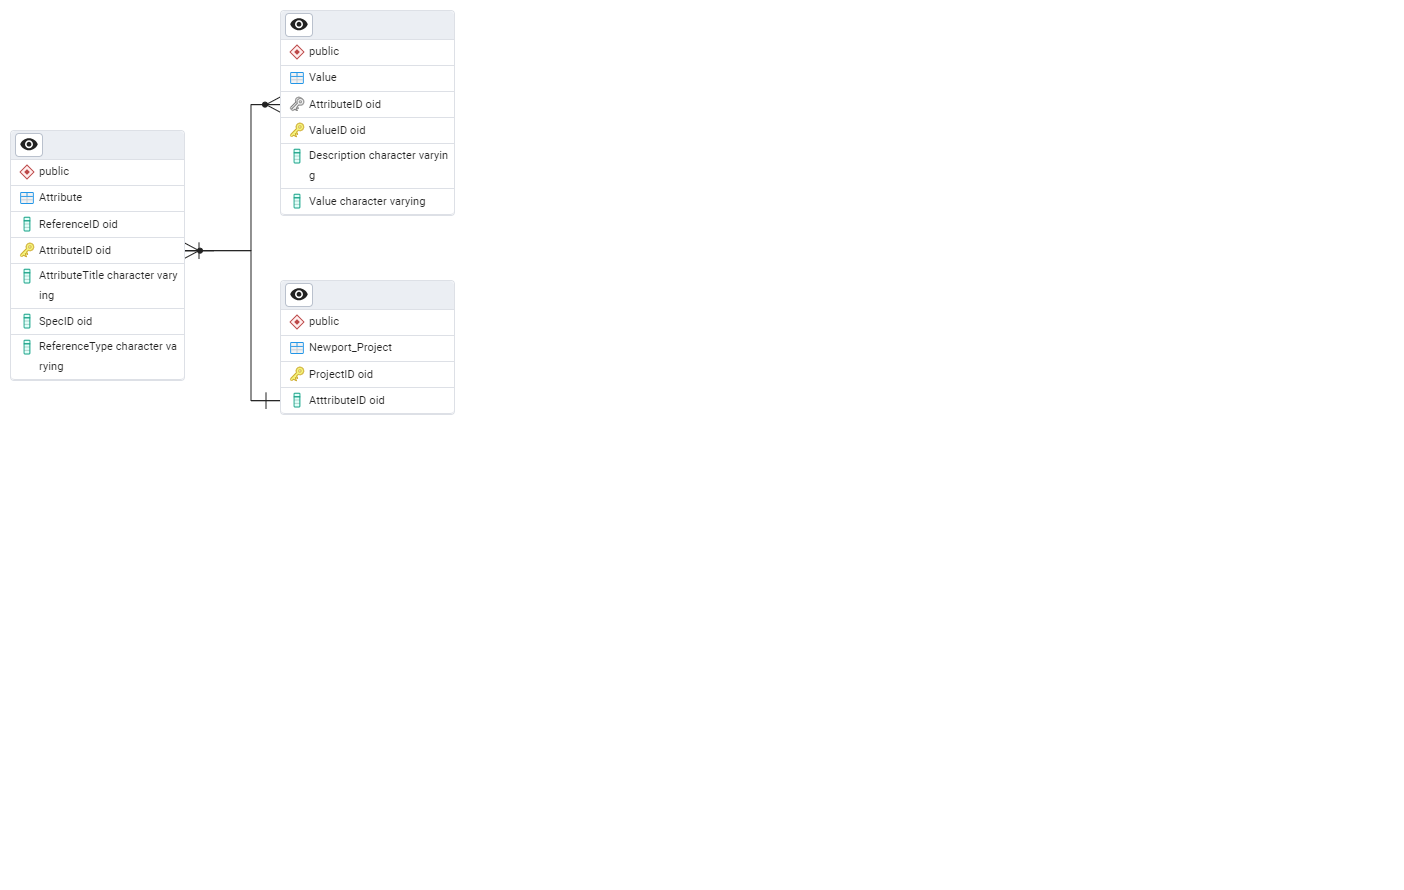
\includegraphics{C:/Bachelor/latex-thesis-template/img/avpmGraphic.png}
\subsection{Technologischer Rahmen}
Um dieses Modell im Backend umzusetzen, und dann im Front-End nutzbar zu machen, bedarf es verschiedener Technologien.
Im Backend werden die Daten in einer Aurora PostgreSQL Datenbank gespeichert\footnote{Diese Wahl beruht auf Standards im Unternehmen. Dazu mehr in der Evaluierung}. 
Aurora PostgreSQL (Im Folgenden Aurora) ist ein Dienst, der die Erstellung von relationalen Datenbanken ermöglicht. Auf dieser relationalen Datenbank ermöglicht eine 
in NodeJS \footnote{Bessere Kompatibilität mit React als alternativen} erstellte API den Zugriff auf und die Bearbeitung der gespeicherten Daten.
Auf diese API greift dann widerum eine React-App zu, die dann ermöglicht, durch eine Benutzeroberfläche die API zur Kommunikation mit der Datenbank zu benutzen.
Die Architektur ist bewusst mehrgliedrich gehalten, um Erweiterungen wie Daten-Redundanz zu ermöglichen \footnote{Unter anderem sollen die Daten in ein großes Daten
Warehouse der Bayer Cropscience kopiert werden} Die Wahl dieses technologischen Rahmens beruht auf vorhandenem Wissen und Infrastruktur im Unternehmen, sowie auch 
Abwägung der Entwicklungsgeschwindigkeit. Grundsätzlich stehen Enwticklern in der Web-Entwicklung jedoch viele Möglichkeiten zur Verfügung
\subsection{Alternative Technologien}
Für die Datenbank wäre es denkbar gewesen, anstatt einer relationalen auf eine sogenannte NoSQL Datenbanken zurückzugreifen. Eine solche Lösung
wird auch im AWS-System angeboten. Der Grund, warum sich gegen diese Option entschieden wurde, liegt in der Natur der Datengrundlage. NoSQL eignet sich vor allem für 
große Mengen unstrukturierter Daten, während traditionelle Datenbanken besser mit strukturierten Daten umgehen können \footnote{nosql source}
Im Rahmen der Anwendung muss zwingendermaßen eine strenge Typisierung von Daten gegeben sein, da auf dessen Basis unter anderem Grafiken erstellt werden sollen. 
Aus diesem Grund ist eine strukturierte Datenbank für den speziellen Zweck des Projekts besser geeignet. 
\break
Die Entscheidung, NodeJS für die API zu verwenden, beruht hauptsächlich auf der zeitlichen Komponente der Entwicklung. React basiert auf einem NodeJS-Environment, weshalb
es sich anbietet, die gleiche Umgebung für die APi zu verwenden. Grundsätzlich hätte auch jede andere Umgebung zur API-Erstellung ihren Zweck erfüllt, und diese Entscheidung 
beruht eher auf Bequemlichkeit. React hingegen als Umgebung wurde mit dem Hintergedanken der Modularität gewählt. Da das Projekt nicht nur eine einzene Anwendung, sondern eher 
einen Komplex kleinerer Tools beherbergen soll, bietet sich ein modulares Framework wie React an, wodurch dieses schon zu Beginn als Anforderung feststand, und als Basis 
aller weiteren Entscheidungen verwendet wurde. Zudem wird React unternehmensintern immer häufiger für verschiedenste Anwendungen verwendet, weshalb die Infrastruktur für das 
Deployment bereits aufgebaut ist. 


\include{chapter/Zusammenfassung}
	
%%%%%%%%%%%%%%%%%%%%%%%%%%%%%%%%%%%%%%%%%%%%%%%%%%%%%%%%%%%%%%%%%%%%%%%

%!TEX root = ../Thesis.tex
\section*{Anhang}
\addcontentsline{toc}{section}{Anhang}
\fancyhead[R]{Anhang}

\anhangsverzeichnis

\anhang{Gesprächsnotizen}

\subanhang{Gespräch mit Werner Müller}

Gespräch mit Werner Müller am 01.01.2013 zum Thema XXX:
\begin{compactitem}
   \item Über das gute Wetter gesprochen
   \item Die Regenwahrscheinlichkeit liegt immer bei ca. 3\%
   \item Das Unternehmen ist total super
   \item Hier könnte eine wichtige Gesprächsnotiz stehen
\end{compactitem}


\anhang{Abbildungen}
\begin{figure}[h]
    \centering
    
\includegraphics[width=5cm]{./img/projektGrafik.png}
    \caption{projektGrafik}
\end{figure}

\anhang{Listings}
\begin{figure}[H]
    \begin{lstlisting}[caption=JS-Code for the LogIn-Button, breaklines = true, label=list:loginbutton]
        // components/LoginButton.js
        import React from 'react';
        import { useAuth } from '../context/AuthContext';
        import { Button } from '@element/react-components';

        export default function LoginButton() {
            const { login } = useAuth();

            return <Button onClick={login} label="Log In"/>
        }
    \end{lstlisting}
    %\footnoterule{}
    %\footnotesize{Casts have been omitted for the sake of readability}
\end{figure}

\begin{figure}[H]
    \begin{lstlisting}[caption=JS-Code for the LogOut-Button, breaklines = true, label=list:logoutbutton]
        // components/LogoutButton.js
        import React from 'react';
        import { useAuth } from '../context/AuthContext';
        import { Button } from '@element/react-components';

        export default function LogoutButton() {
            const { logout } = useAuth();

            return <Button onClick={logout} label="Log Out"/>
        }
    \end{lstlisting}
    %\footnoterule{}
    %\footnotesize{Casts have been omitted for the sake of readability}
\end{figure}

\begin{figure}[H]
    \begin{lstlisting}[caption=JS-Code for the AuthButton, breaklines = true, label=list:authbutton]
        // components/AuthButton.js
        import React from 'react';
        import { useAuth } from '../context/AuthContext';
        import LoginButton from './LoginButton';
        import LogoutButton from './LogoutButton';

        export default function AuthButton() {
            const { isAuthenticated } = useAuth();

            return isAuthenticated ? <LogoutButton /> : <LoginButton />;
        }
    \end{lstlisting}
    %\footnoterule{}
    %\footnotesize{Casts have been omitted for the sake of readability}
\end{figure}

\begin{figure}[H]
    \begin{lstlisting}[caption=Import und Kontext, breaklines = true, label=list:authcontextimports]
        import React, { createContext, useState, 
        useEffect, useContext } from 'react';
        import { useNavigate, useLocation } from 'react-router-dom';
        import {buildAuthUrl, generateChallenge, generateVerifier, 
        exchangeCodeForTokens} from '../service/authService';
        import authConfig from '../services/authConfig';
        import {generateVerifier, generateChallenge} from '../service/pkce';

        const AuthContext = createContext();
    \end{lstlisting}
\end{figure}

\begin{figure}[H]
    \begin{lstlisting}[caption=Variablen für den Authentifizierungs-Kontext, breaklines = true, label=list:authcontextvariables]
        const [user, setUser] = useState(null);
        const [isAuthenticated, setIsAuthenticated] = useState(false);
        const [tokens, setTokens] = useState(null);
        const navigate = useNavigate();
        const location = useLocation();
    \end{lstlisting}
\end{figure}

\begin{figure}[H]
    \begin{lstlisting}[caption=Login-Methode, breaklines = true, label=list:authcontextlogin]
        async function login() {
            const state = crypto.randomUUID();
            const verifier = generateVerifier();
            const challenge = await generateChallenge(verifier);

            sessionStorage.setItem('oauth_state', state);
            sessionStorage.setItem('pkce_verifier', verifier);
            
            const url = buildAuthUrl({state, code_challenge: challenge});

            window.location.href = url;
        }
\end{lstlisting}
\end{figure}

\begin{figure}[H]
    \begin{lstlisting}[caption=Logout-Methode, breaklines = true, label=list:authcontextlogout]
        function logout() {
            sessionStorage.clear();
            const {logoutEndpoint, clientId, logoutUri} =authConfig;
            window.location.href = `${logoutEndpoint}?client_id=${clientId}&logout_uri=${encodeURIComponent(logoutUri)}`; 
        }
    \end{lstlisting}
\end{figure}

\begin{figure}[H]
    \begin{lstlisting}[caption=Callback-Handling, breaklines = true, label=list:authcontextcallback]
        useEffect(() => {
            if (location.pathname === '/callback' && location.search.includes('code=')) {
                handleCallback();
            }
        }, [location, handleCallback]);
\end{lstlisting}
\end{figure}

\begin{figure}[H]
    \begin{lstlisting}[caption=Callback-Handling, breaklines = true, label=list:authcontextcallback2]
        async function handleCallback() {
            const params = new URLSearchParams(location.search);
            const code = params.get('code');
            const state = params.get('state');
            const saved = sessionStorage.getItem('oauth_state');

            if(!code || !state || state !== saved) {
                return navigate('/', {replace: true});
            }

            try{
                const verifier = sessionStorage.getItem('pkce_verifier');
                const tokenSet = await exchangeCodeForTokens(code, verifier);
                setTokens(tokenSet);

                const [, payload] = tokenSet.id_token.split('.');
                const userInfo = JSON.parse(atob(payload));
                setIsAuthenticated(true);

                sessionStorage.removeItem('pkce_verifier');
                sessionStorage.removeItem('oauth_state');

                navigate('/dashboard', {replace: true});
            } catch (err) {
                console.error('Error during authentication:', err);
                navigate('/', {replace: true});
            }
        }
    \end{lstlisting}
\end{figure}

\begin{figure}[H]
    \begin{lstlisting}[caption=AuthProvider-Komponente, breaklines = true, label=list:authcontextprovider]
        return (
            <AuthContext.Provider 
            value={{ user, isAuthenticated, tokens, login, logout }}>
                {children}
            </AuthContext.Provider>
        );
    }
    export function useAuth() {
        return useContext(AuthContext);
    }
    \end{lstlisting}
\end{figure}

\begin{figure}[H]
    \begin{lstlisting}[caption=AuthConfig, breaklines = true, label=list:authconfig]
        const domain = process.env.REACT_APP_COGNITO_DOMAIN;
        const clientId = process.env.REACT_APP_COGNITO_CLIENT_ID; 
        const redirectUri = process.env.REACT_APP_COGNITO_REDIRECT_URI;
        const logoutUri = process.env.REACT_APP_COGNITO_LOGOUT_URI;
        const apiBaseUrl = process.env.REACT_APP_API_BASE_URL;
        export const authConfig = {
            domain,
            clientId,
            redirectUri,
            logoutUri,
            apiBaseUrl: apiBaseUrl,
            authEndpoint: `https://${domain}/oauth2/authorize`,
            tokenEndpoint: `https://${domain}/oauth2/token`,
            logoutEndpoint: `https://${domain}/logout`,
            responseType: 'code',
            scope: 'openid profile email',
        };
    \end{lstlisting}
\end{figure}

\begin{figure}[H]
    \begin{lstlisting}[caption=Build-Auth Methode, breaklines = true, label=list:buildAuth]
        export function buildAuthUrl({state, code_challenge}) {
            const {
                authorizeEndpoint,
                clientId,
                redirectUri,
                responseType,
                scope
            } = authConfig;
            const params = new URLSearchParams({
                client_id: clientId,
                redirect_uri: redirectUri,
                response_type: responseType,
                scope,
                state,
                code_challenge_method: 'S256',
                code_challenge
            });
            return '${authorizeEndpoint}?{params}';
        }
    \end{lstlisting}
\end{figure}

\begin{figure}[H]
    \begin{lstlisting}[caption=ExchangeCodeForToken Methode, breaklines = true, label=list:exchangecodefortoken]
        export async function exchangeCodeForToken(code, code_verifier){
            const {tokenEndpoint, clientId, redirectUri} = authConfig;

            const params = new URLSearchParams({
                grant_type: 'authorization_code',
                client_id: clientId,
                code,
                redirect_uri: redirectUri,
                code_verifier
            });

            const resp = await fetch(tokenEndpoint, {
                method: 'POST',
                headers: {'Content-Type': 'application/x-www-form-urlencoded' },
                body: params.toString()
            });

            const text = await resp.text();

            if(!resp.ok) throw new Error('Token Exchange failed: $(text)')
            return JSON.parse(text);
        }
    \end{lstlisting}
\end{figure}

\begin{figure}[H]
    \begin{lstlisting}[caption=PKCE-Verifier-Generierung, breaklines = true, label=list:pkceverifier]
        export function generateVerifier() {
            const array = new Uint8Array(32);	
            crypto.getRandomValues(array);
            return Array.from(array, b => ('0'+ b.toString(16)).slice(-2)).join('');
        }
    \end{lstlisting}
\end{figure}

\begin{figure}[H]
    \begin{lstlisting}[caption=PKCE-Challenge-Generierung, breaklines = true, label=list:pkcechallenge]
        export async function generateChallenge(verifier) {
            const encoder = new TextEncoder();
            const data = encoder.encode(verifier);
            const hash = await crypto.subtle.digest('SHA-256', data);
            return btoa(String.fromCharCode(...new Uint8Array(hash)))
                .replace(/\+/g, '-').replace(/\//g, '_').replace(/=+$/, '');
        }
    \end{lstlisting}
\end{figure}

\begin{figure}[H]
    \begin{lstlisting}[caption=PKCE-Challenge-Generierung, breaklines = true, label=list:callApi]
        async function callApi(path, options = {}){
            const url = '${authConfig.apiBaseUrl}${path}';
            const resp = await fetch(url, {
                ...options,
                headers: {
                    'Content-Type': 'application/json',
                    Authorization: 'Bearer ${tokens.access_token}',
                    ...options, headers
                }
            });
            if (!resp.ok) throw 
            new Error('API error ${resp.status}: ${await resp.text()}');
            return resp.json();
        }
    \end{lstlisting}
\end{figure}

\include{chapter/Quellenverzeichnis}


%%%%%%%%%%%%%%%%%%%%%%%%%%%%%%%%%%%%%%%%%%%%%%%%%%%%%%%%%%%%%%%%%%%%%%%

\include{chapter/Ehrenwoertliche_Erklaerung}
 
%%%%%%%%%%%%%%%%%%%%%%%%%%%%%%%%%%%%%%%%%%%%%%%%%%%%%%%%%%%%%%%%%%%%%%%

\end{document}